\documentclass{article}

\usepackage{import}
\subimport{preamble/}{lab_preamble.tex}

\title{Passive Analog Signal Processing}


\begin{document}
\maketitle

In this chapter we introduce filters and signal transmission theory. Filters are essential components of most analog circuits and are used to remove unwanted signals (i.e. noise) from the actual signal. Transmission lines are essential for sending signals from one device to another, such as from a detector to a data acquisition module.

\section{Filters}
Filters are ubiquitous in analog electronic circuitry. In fact, if you see a capacitor or an inductor in a circuit there is a good chance it is part of a filter. Filters are frequently used to clean up (i.e. remove high frequency noise) power supplies and remove spurious frequencies from a signal (frequently  60\,Hz, switching power supply noise in computers, display screen noise, ground loop noise, and Radio-Frequency (RF) pick-up).

\subsection{RC Filters}
RC filters are by far the most common filters around. They are simple to make (i.e. just a resistor and a capacitor), reliable, and involve relatively simple design calculations.

\subsubsection{The Low-Pass RC Filter}

\begin{figure}
 \begin{center}
  \begin{circuitikz}
   \draw (-2,2) node[left]{$v_{in}$} to[R,l=$R$,o-] (0,2) to[C,l=$C$] (0,0) node[ground]{};
   \draw (0,2) to[short,-o] (1,2) node[right]{$v_{out}$};
  \end{circuitikz}
  \caption{Low-pass RC filter circuit.}
  \label{fig:rc_low_pass_filter}
 \end{center}
\end{figure}

The low-pass RC filter, or integrator, is used to remove high frequencies from a signal. Applications include the removal of RF pick-up noise and reducing ripple voltages on power supplies.

A generic RC low pass filter circuit is shown in Figure~\ref{fig:rc_low_pass_filter}. We have already calculated its performance in the previous lab using Fourier analysis and complex impedances. We recall the results:
\begin{equation}
v_{out} = v_C = v_0 \sin\phi e^{j(\omega t + \phi - \pi/2)}
\end{equation}
where $\sin\phi = 1/\sqrt{1 + (\omega R C)^2}$ and $v_{in} = v_0 e^{j \omega t}$. From these quantities we can compute the magnitude of the gain and the phase performance of the filter. The magnitude of the gain is defined as $|G(\omega)| = |v_{out} / v_{in}|$ and the phase as $\phi - \pi/2$ (this is just the part after the $\omega t$ in the exponent).

The RC filter is just a voltage divider with complex impedances, so we can calculate the gain easily:
\begin{equation}
|G(\omega)| = |v_{out} / v_{in}| = \left|\frac{\frac{1}{j\omega C}}{R + \frac{1}{j\omega C}}\right| = \left|\frac{1}{1+j\omega RC}\right| = \frac{1}{\sqrt{1 + (\omega R C)^2}} = \sin\phi.
\end{equation}
The phase of the output voltage with respect to the input is easily computed and is given by
\begin{equation}
\tan(\phi - \pi/2) = \cot \phi = \omega RC
\end{equation}
At $\omega = 1/RC$, the output voltage drops to $1/\sqrt{2}$ of the input voltage, and consequently the power transmission drops to 50\% or -3\,dB\footnotemark{}. At this frequency, the voltage across the resistor and the voltage across the capacitor are equal in amplitude, but $\pm \pi/4$ out of phase with the drive voltage. The average value of $V^2$ across either the resistor or the capacitor is down by a factor of 2 from the drive voltage. Consequently, this frequency characterizes the RC circuit completely and is called the 3\,dB frequency. We can rewrite the gain and phase equations in terms of the 3\,dB frequency:
\begin{equation}
G(f) = \frac{1}{\sqrt{1 + (f/f_{3\,dB})^2}}
\end{equation}
and
\begin{equation}
\tan\phi = f/f_{3\,dB}
\end{equation}
with $f_{3\,dB} = 1/2\pi RC$.

\footnotetext{A dB or decibel is a notation for quantifying a ratio of two numbers. For power, a dB is defined as
\begin{equation*}
dB = 10 log_{10} \frac{P}{P_0}
\end{equation*}
From this definition we can see that a ratio of 0.5 is roughly -3. Hence -3\,dB is the same as halving a signal. For voltage or current, a dB is defined as
\begin{equation*}
dB = 20 log_{10} \frac{V}{V_0}
\end{equation*}
So at -3\,dB, the voltage (or current) has dropped to $1/\sqrt{2}$ of its input value.}

\begin{figure}
\begin{center}
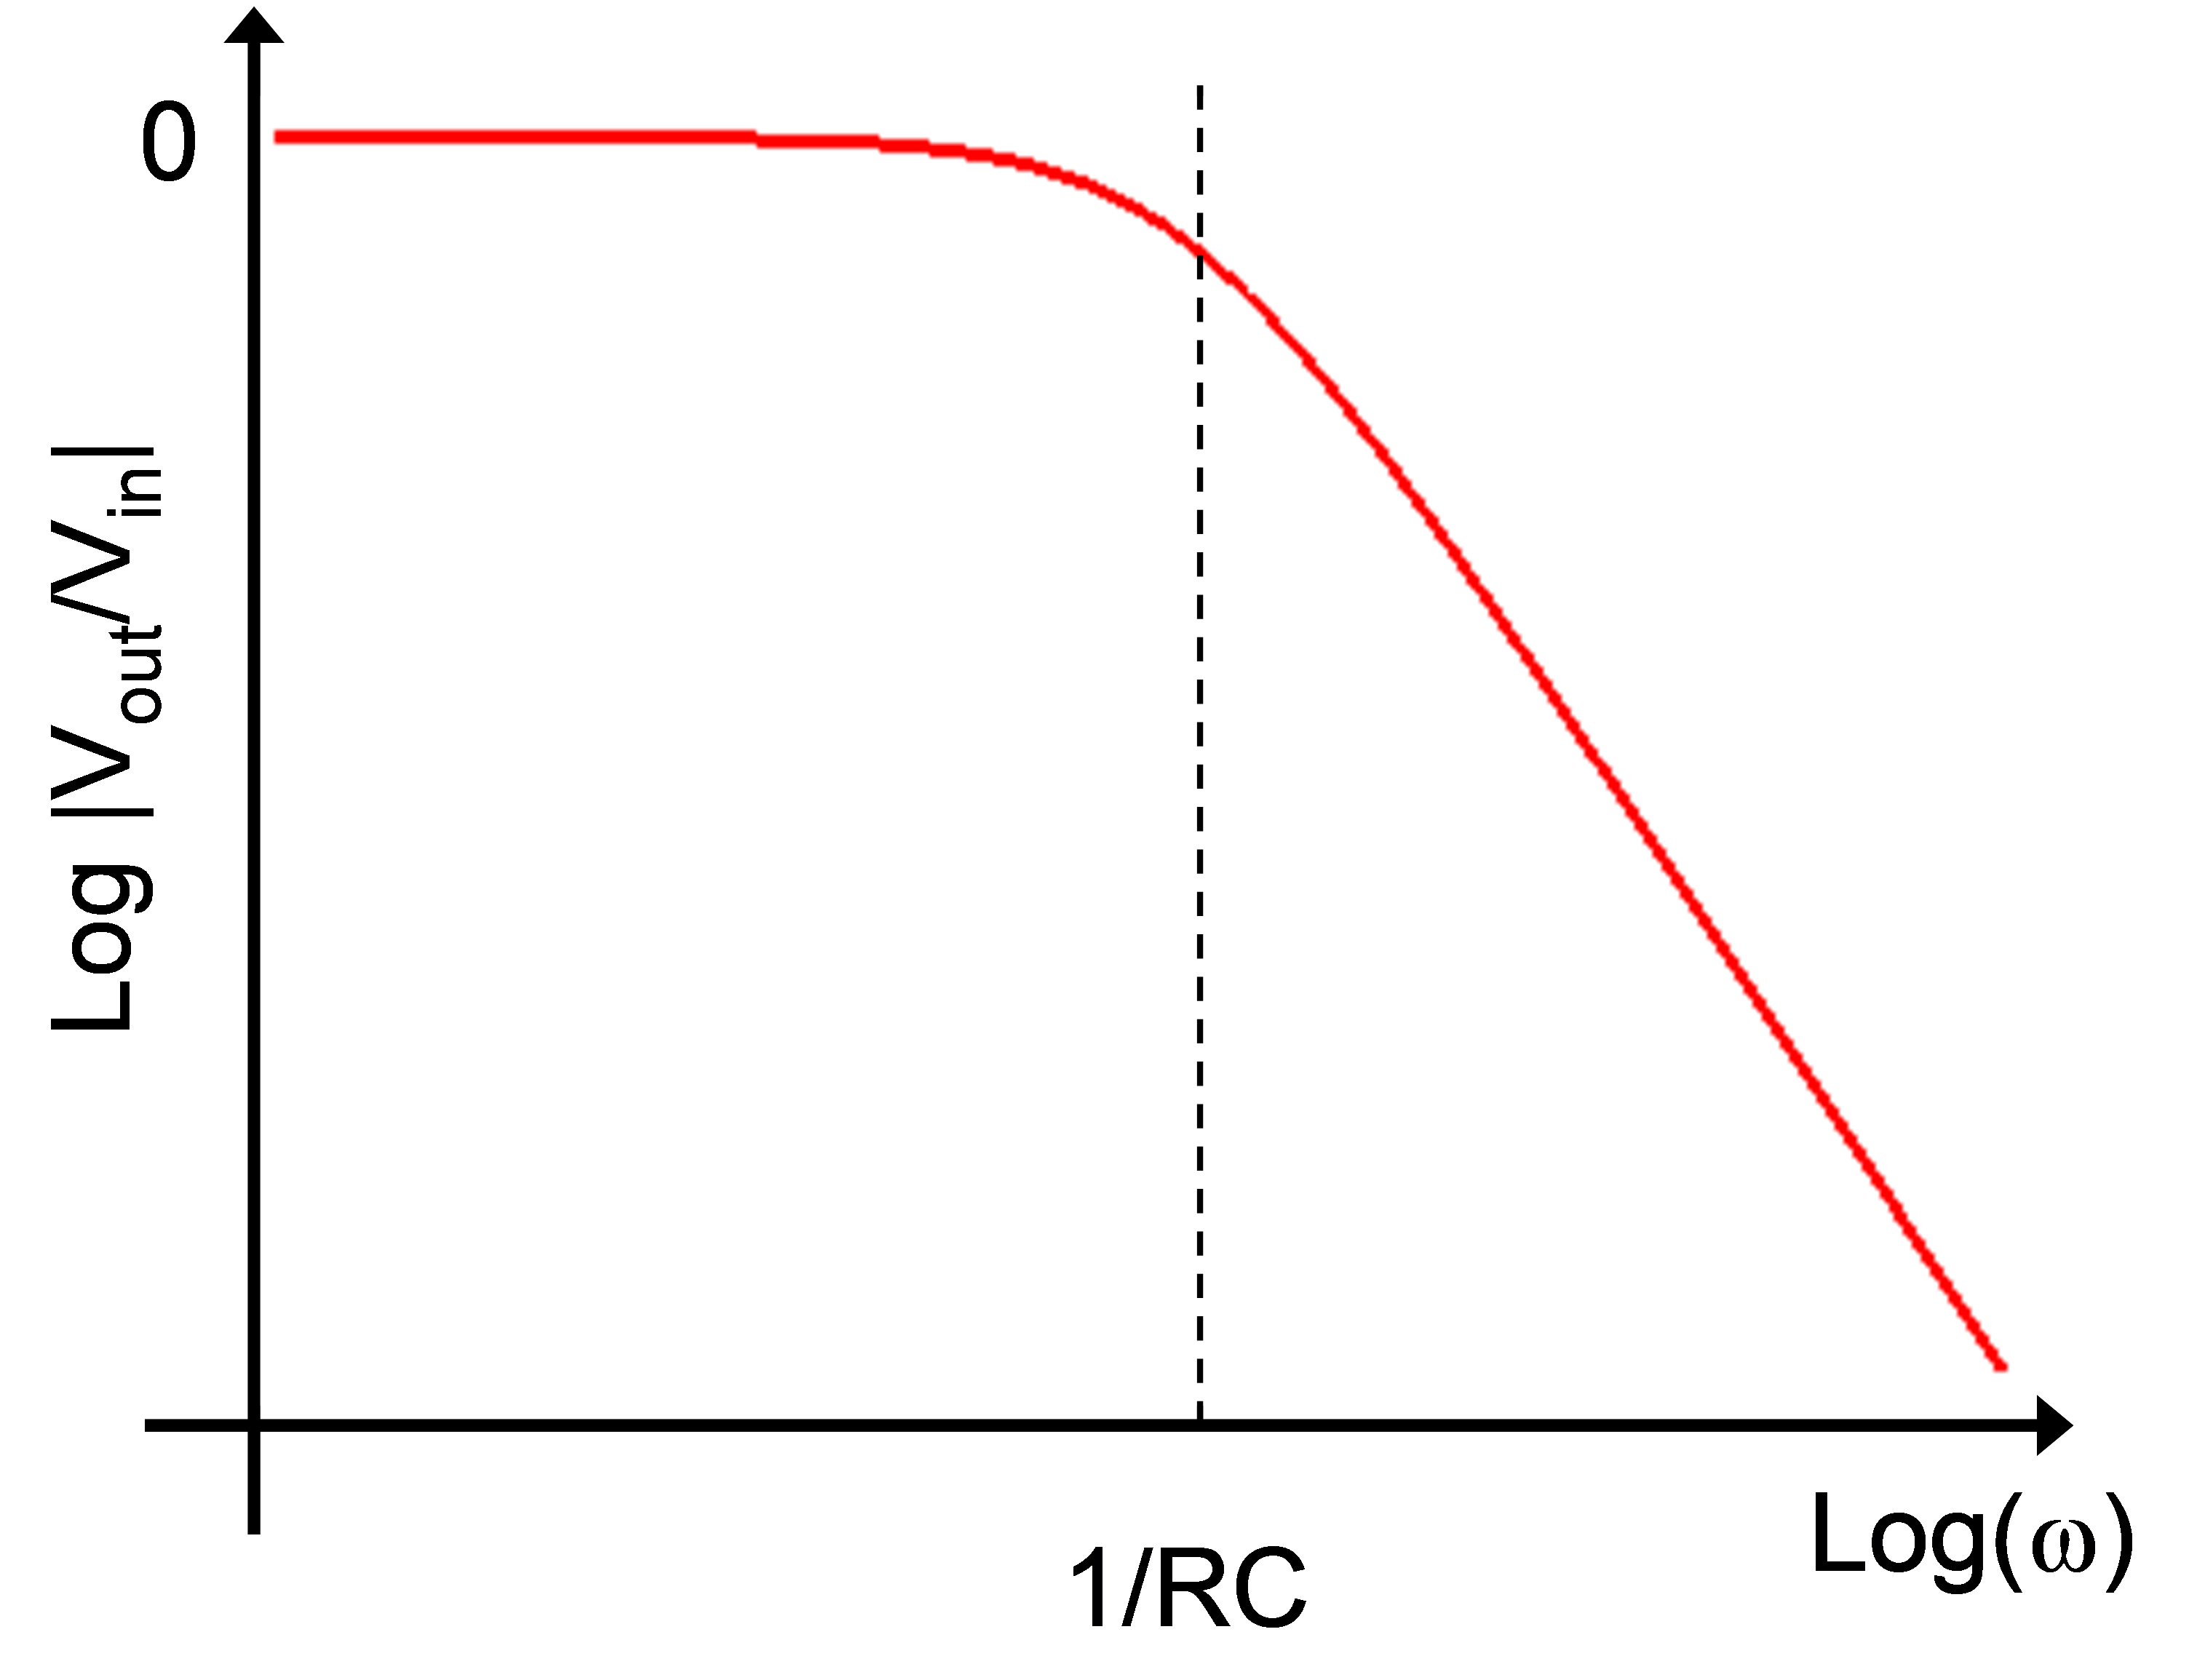
\includegraphics[width=0.45\textwidth]{pics/rc_low_pass_filter_bode_plot_magnitude}
\quad
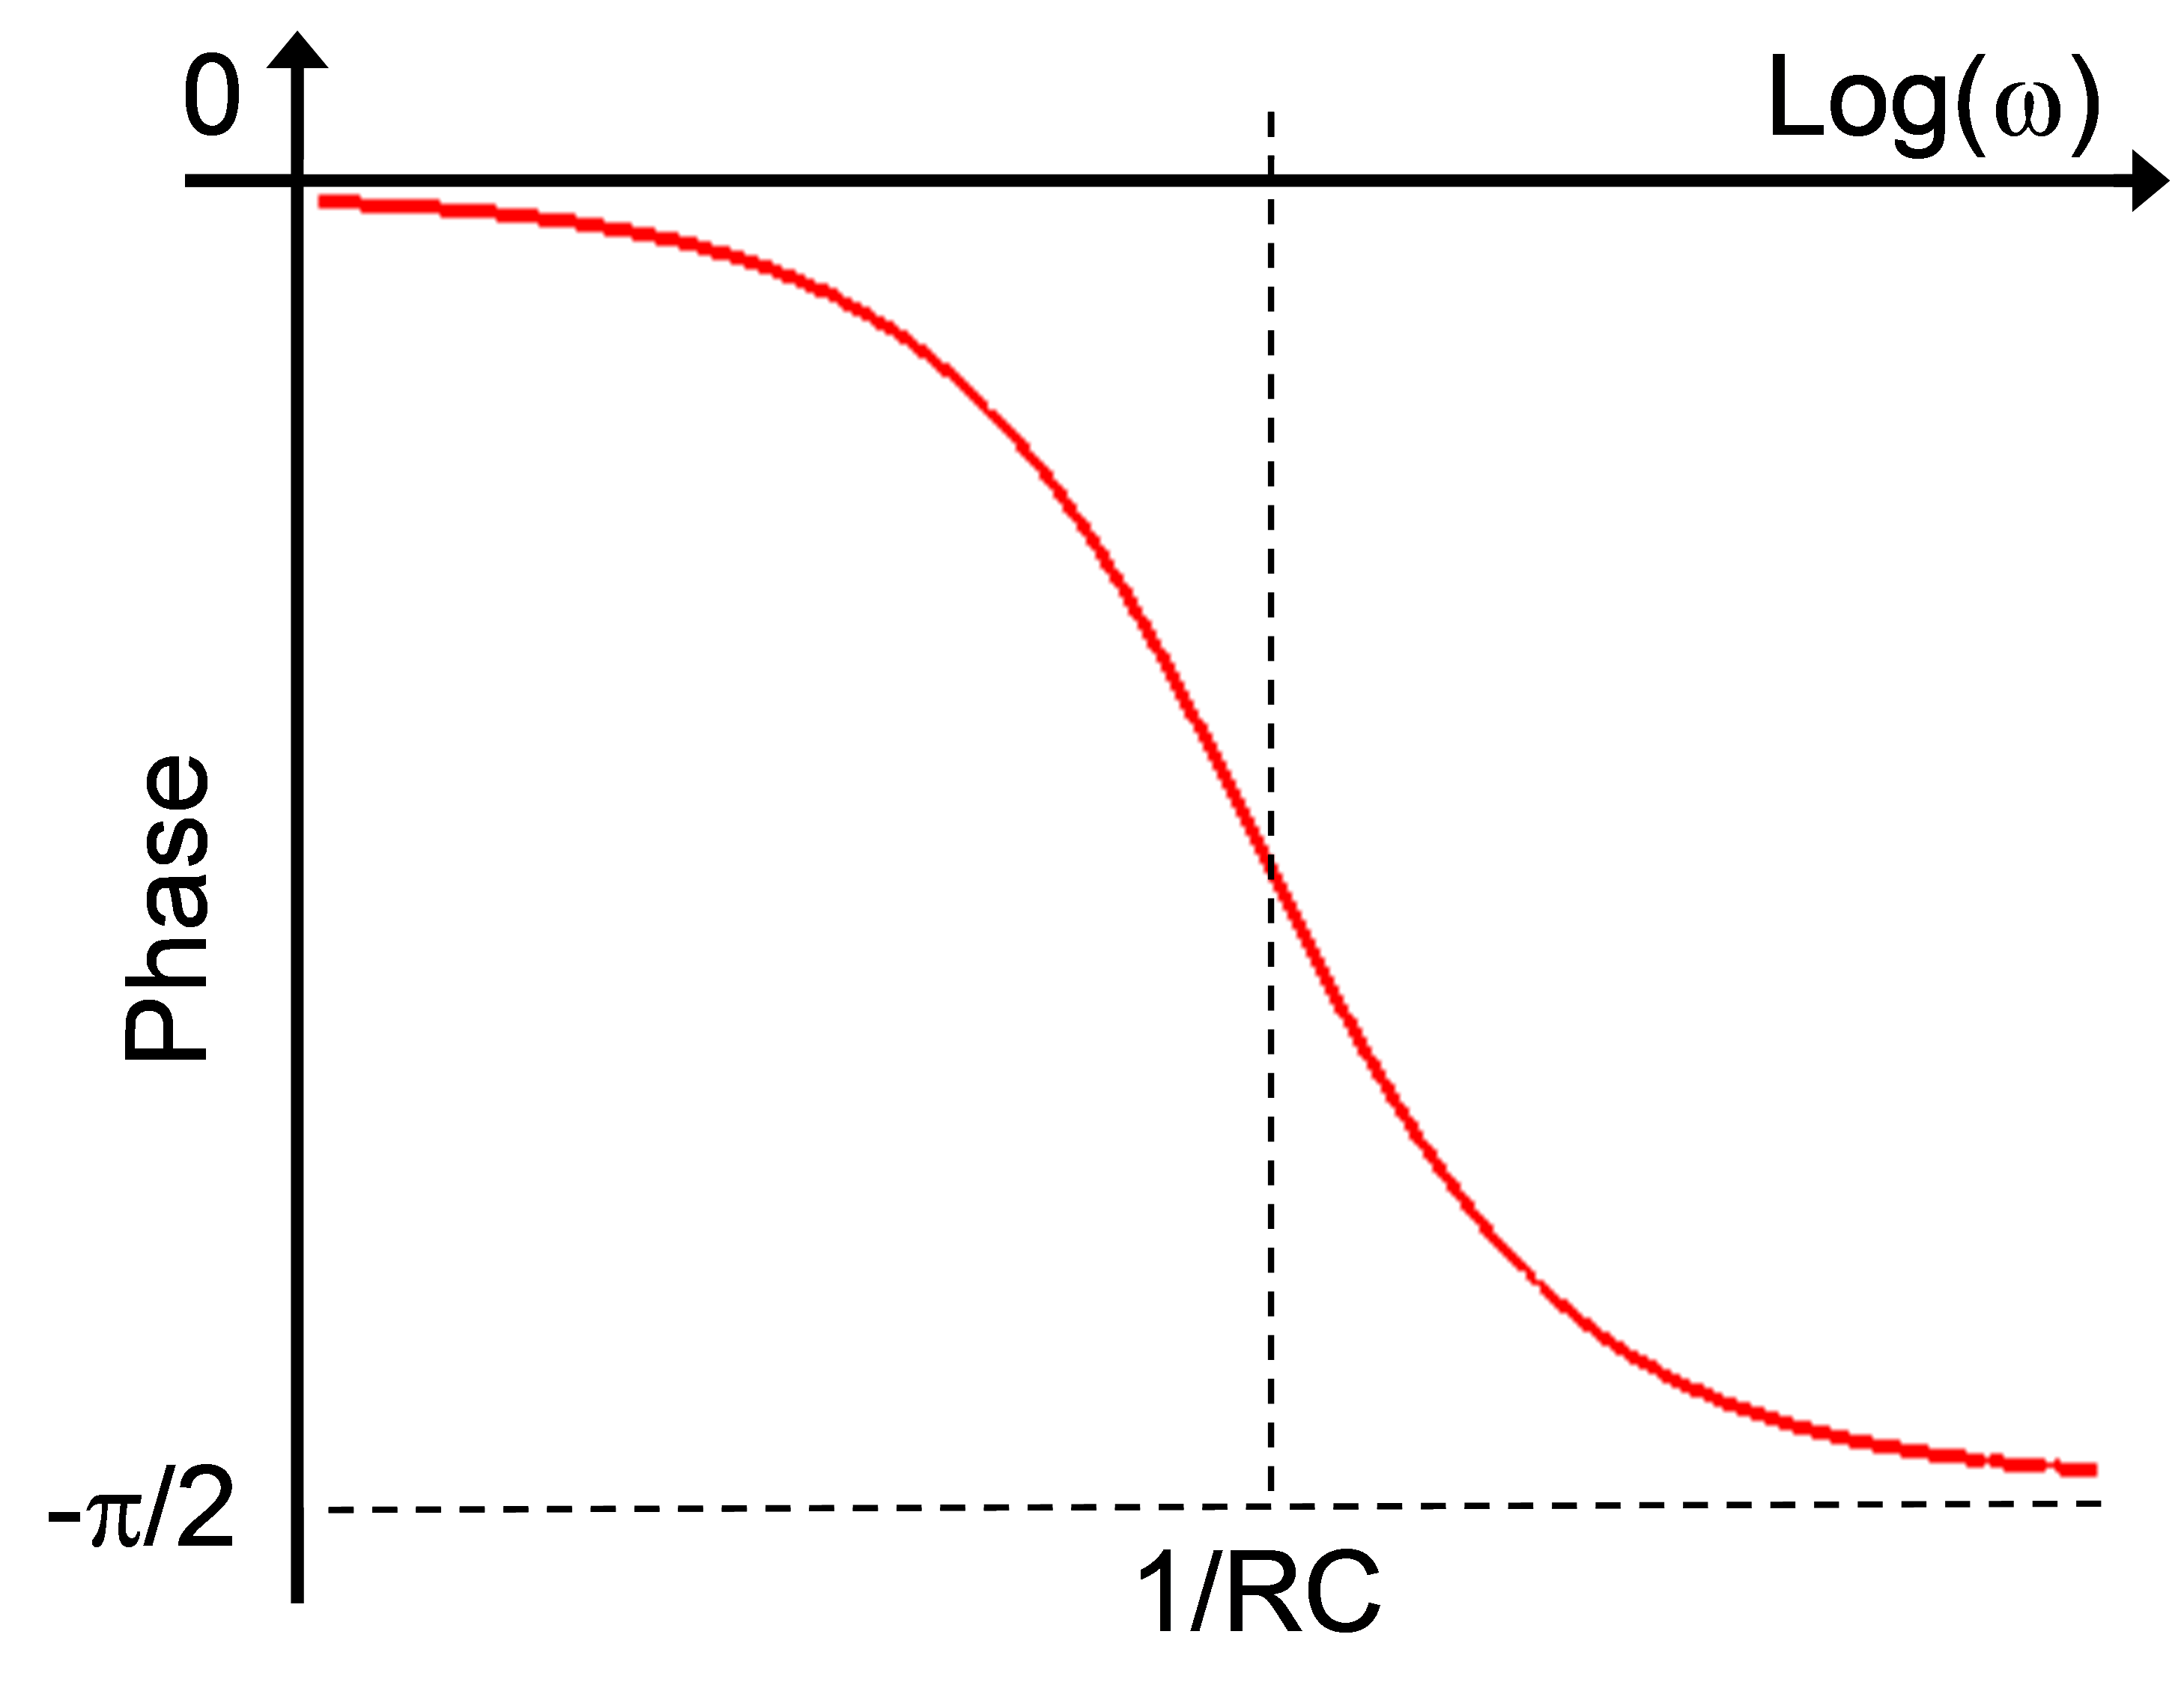
\includegraphics[width=0.45\textwidth]{pics/rc_low_pass_filter_bode_plot_phase}
\end{center}
\caption{Bode plots of the relative magnitude (left) and phase (right) of the output of an RC low-pass filter.}
\label{fig:rc_low_pass_filter_bode_plot}
\end{figure}

The Bode plots (log-log or semi-log plots) for the gain and phase of the low pass filter are shown in Figure~\ref{fig:rc_low_pass_filter_bode_plot}. Past the -3\,dB point, the log-log ``slope'' for the gain is  -20\,dB/decade or -6\,dB/decade.

The low-pass RC filter is also called an integrator because it integrates currents with frequencies above $f_{3\,dB}$. In other words $v_{out} = \frac{1}{C} \int I(t)dt$ (see lab 3) for currents with frequency components above $f_{3\,dB}$.

\subsubsection{The High-Pass RC Filter}

\begin{figure}
 \begin{center}
  \begin{circuitikz}
   \draw (-2,2) node[left]{$v_{in}$} to[C,l=$C$,o-] (0,2) to[R,l=$R$] (0,0) node[ground]{};
   \draw (0,2) to[short,-o] (1,2) node[right]{$v_{out}$};
  \end{circuitikz}
  \caption{High-pass RC filter circuit.}
  \label{fig:rc_high_pass_filter}
 \end{center}
\end{figure}

The high-pass RC filter, or differentiator, is used to remove low frequencies from a signal. Applications include the removal of DC bias voltages and 60\,Hz pick-up voltages.

A generic RC high-pass filter circuit is shown in Figure~\ref{fig:rc_high_pass_filter}. Mathematically, high-pass filter can be treated the same way as their low pass cousins: they are almost identical except that $v_{out}$ measures the voltage drop across the resistor instead of the capacitor. Qualitatively, the capacitor blocks DC and low frequency signals.

If we treat the high-pass filter as a complex impedance voltage divider, then we obtain immediately
\begin{equation}
|G(\omega)| = |v_{out} / v_{in}| = \left|\frac{R}{R + \frac{1}{j\omega C}}\right| = \left|\frac{j\omega RC}{1+j\omega RC}\right| = \frac{\omega RC}{\sqrt{1 + (\omega R C)^2}} = \cos\phi.
\end{equation}
and
\begin{equation}
\tan\phi = \frac{1}{\omega RC}
\end{equation}

We can rewrite these using only $f_{3\,dB}$ to produce more compact design equations:
\begin{equation}
G(f) = \frac{(f/f_{3\,dB})}{\sqrt{1 + (f/f_{3\,dB})^2}}
\end{equation}
and
\begin{equation}
\tan\phi = f_{3\,dB}/f
\end{equation}
with $f_{3\,dB} = 1/2\pi RC$.

\begin{figure}
\begin{center}
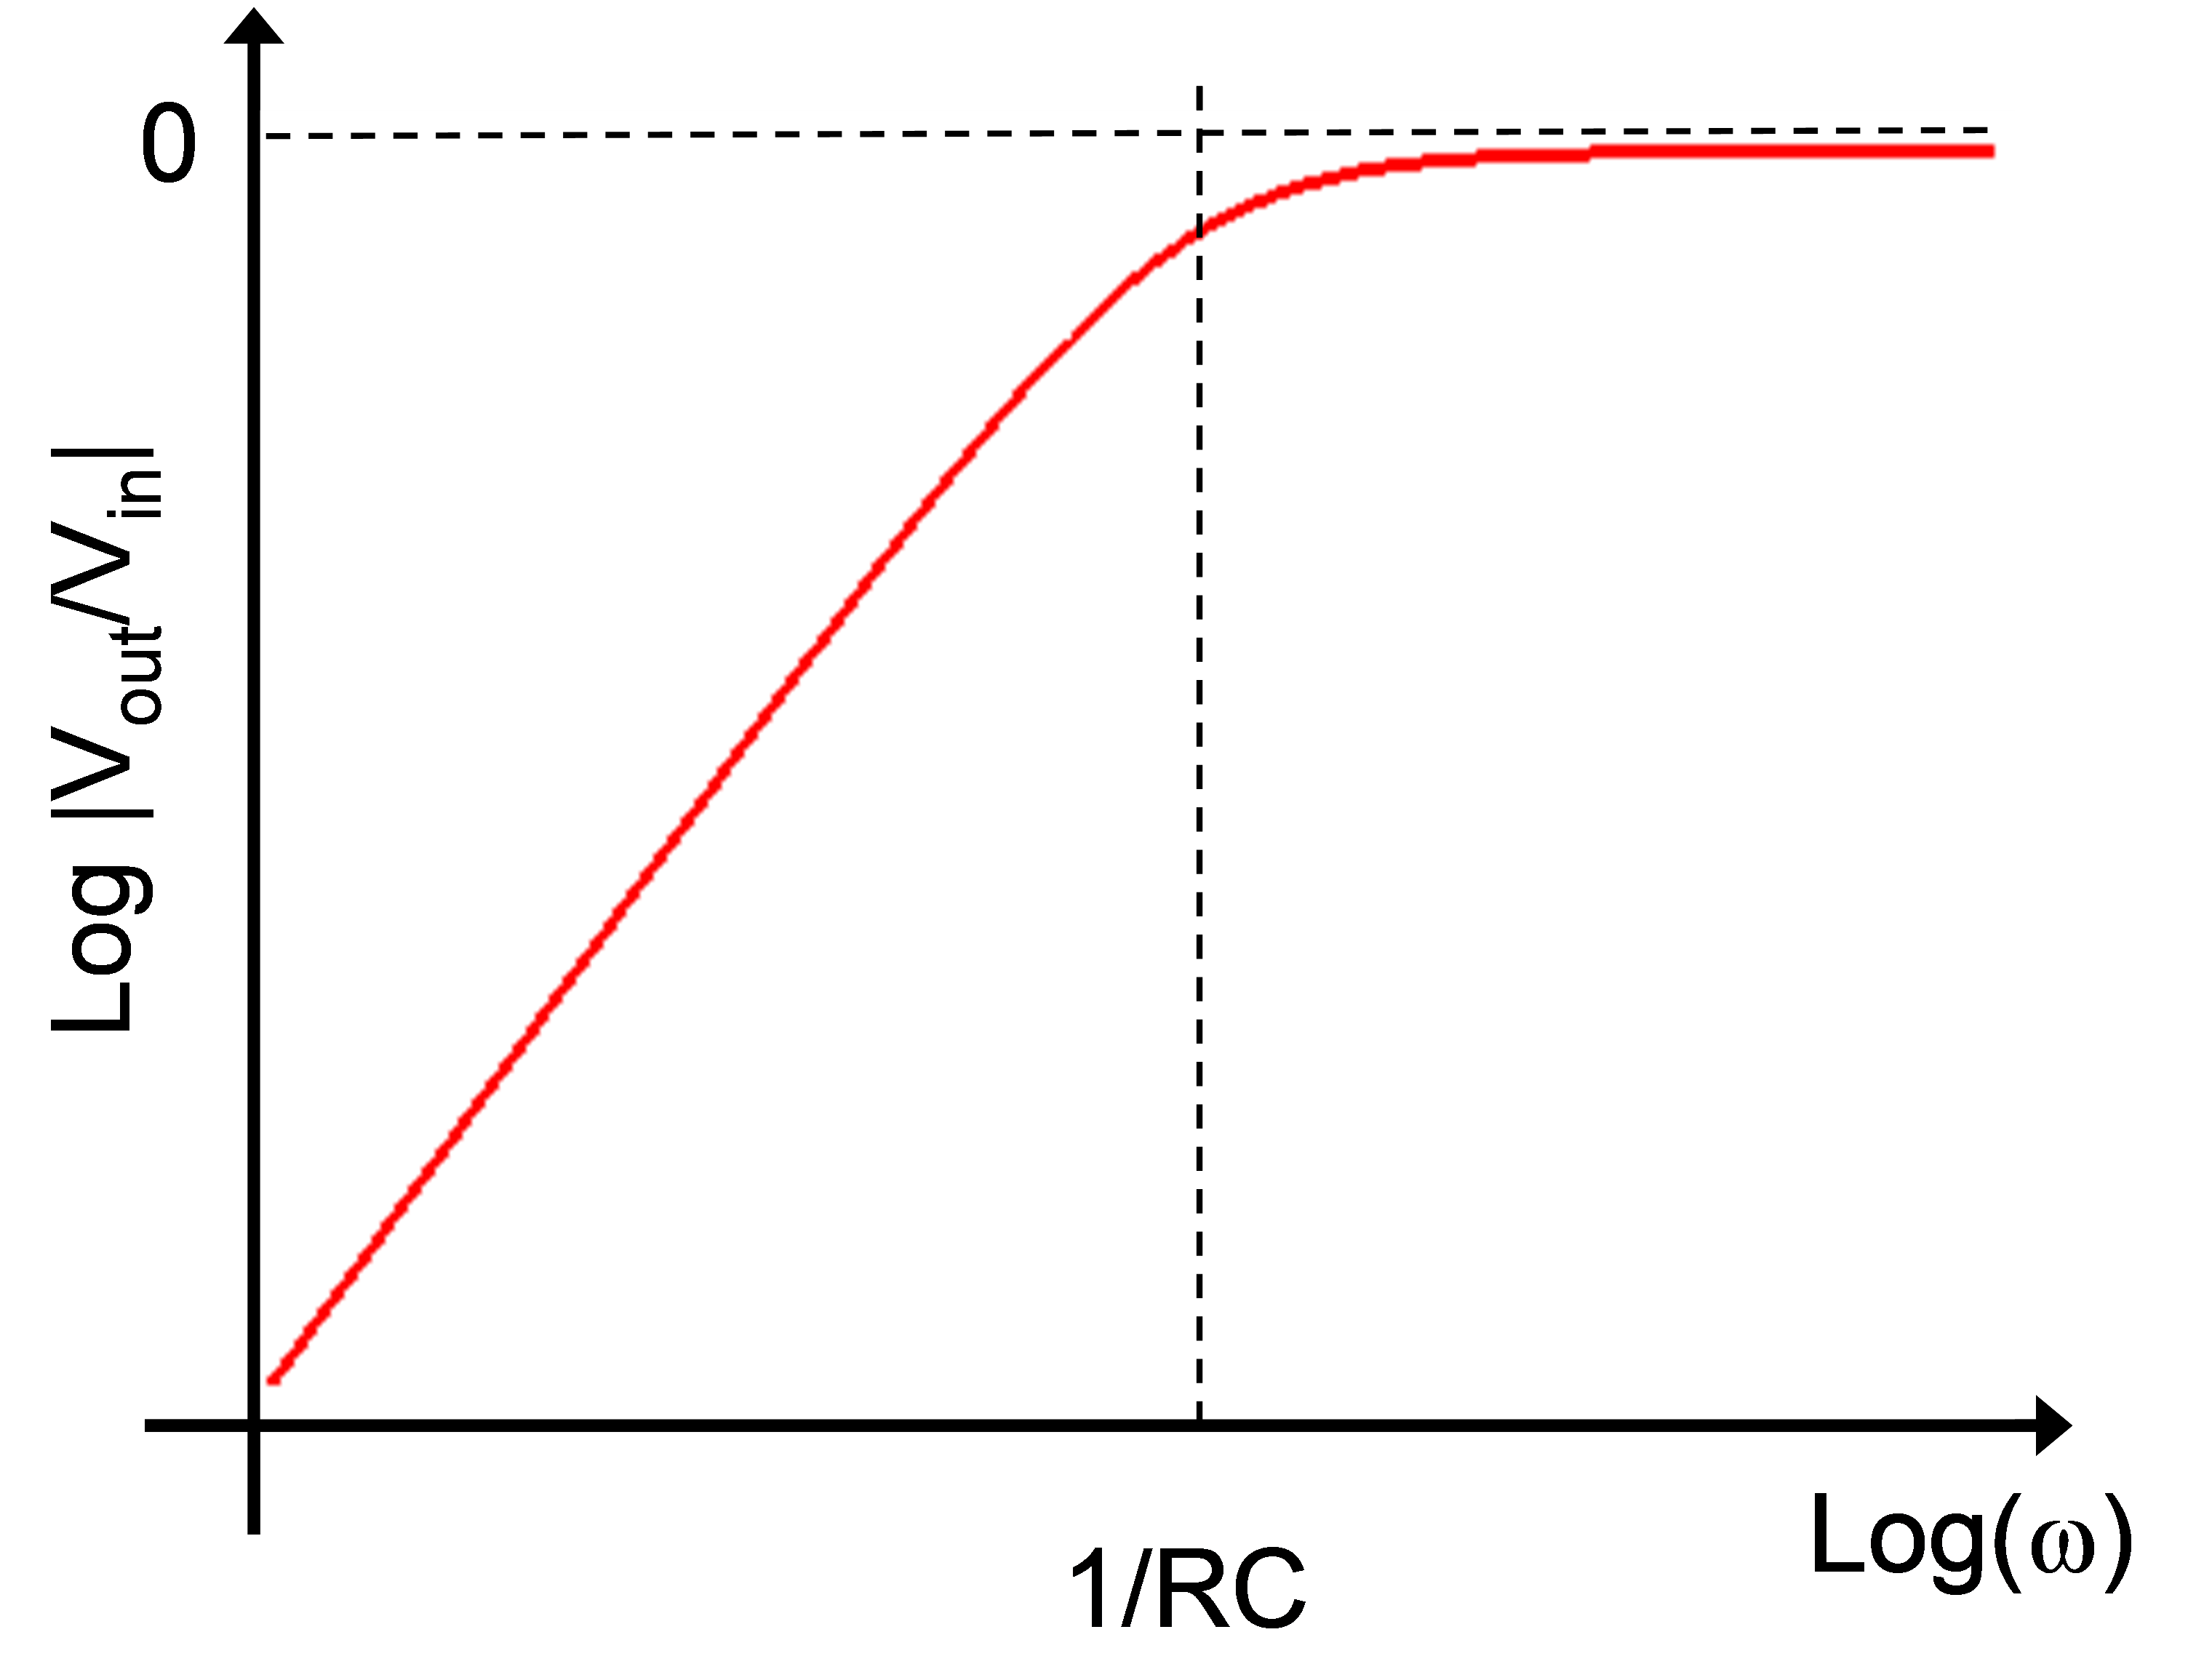
\includegraphics[width=0.45\textwidth]{pics/rc_high_pass_filter_bode_plot_magnitude}
\quad
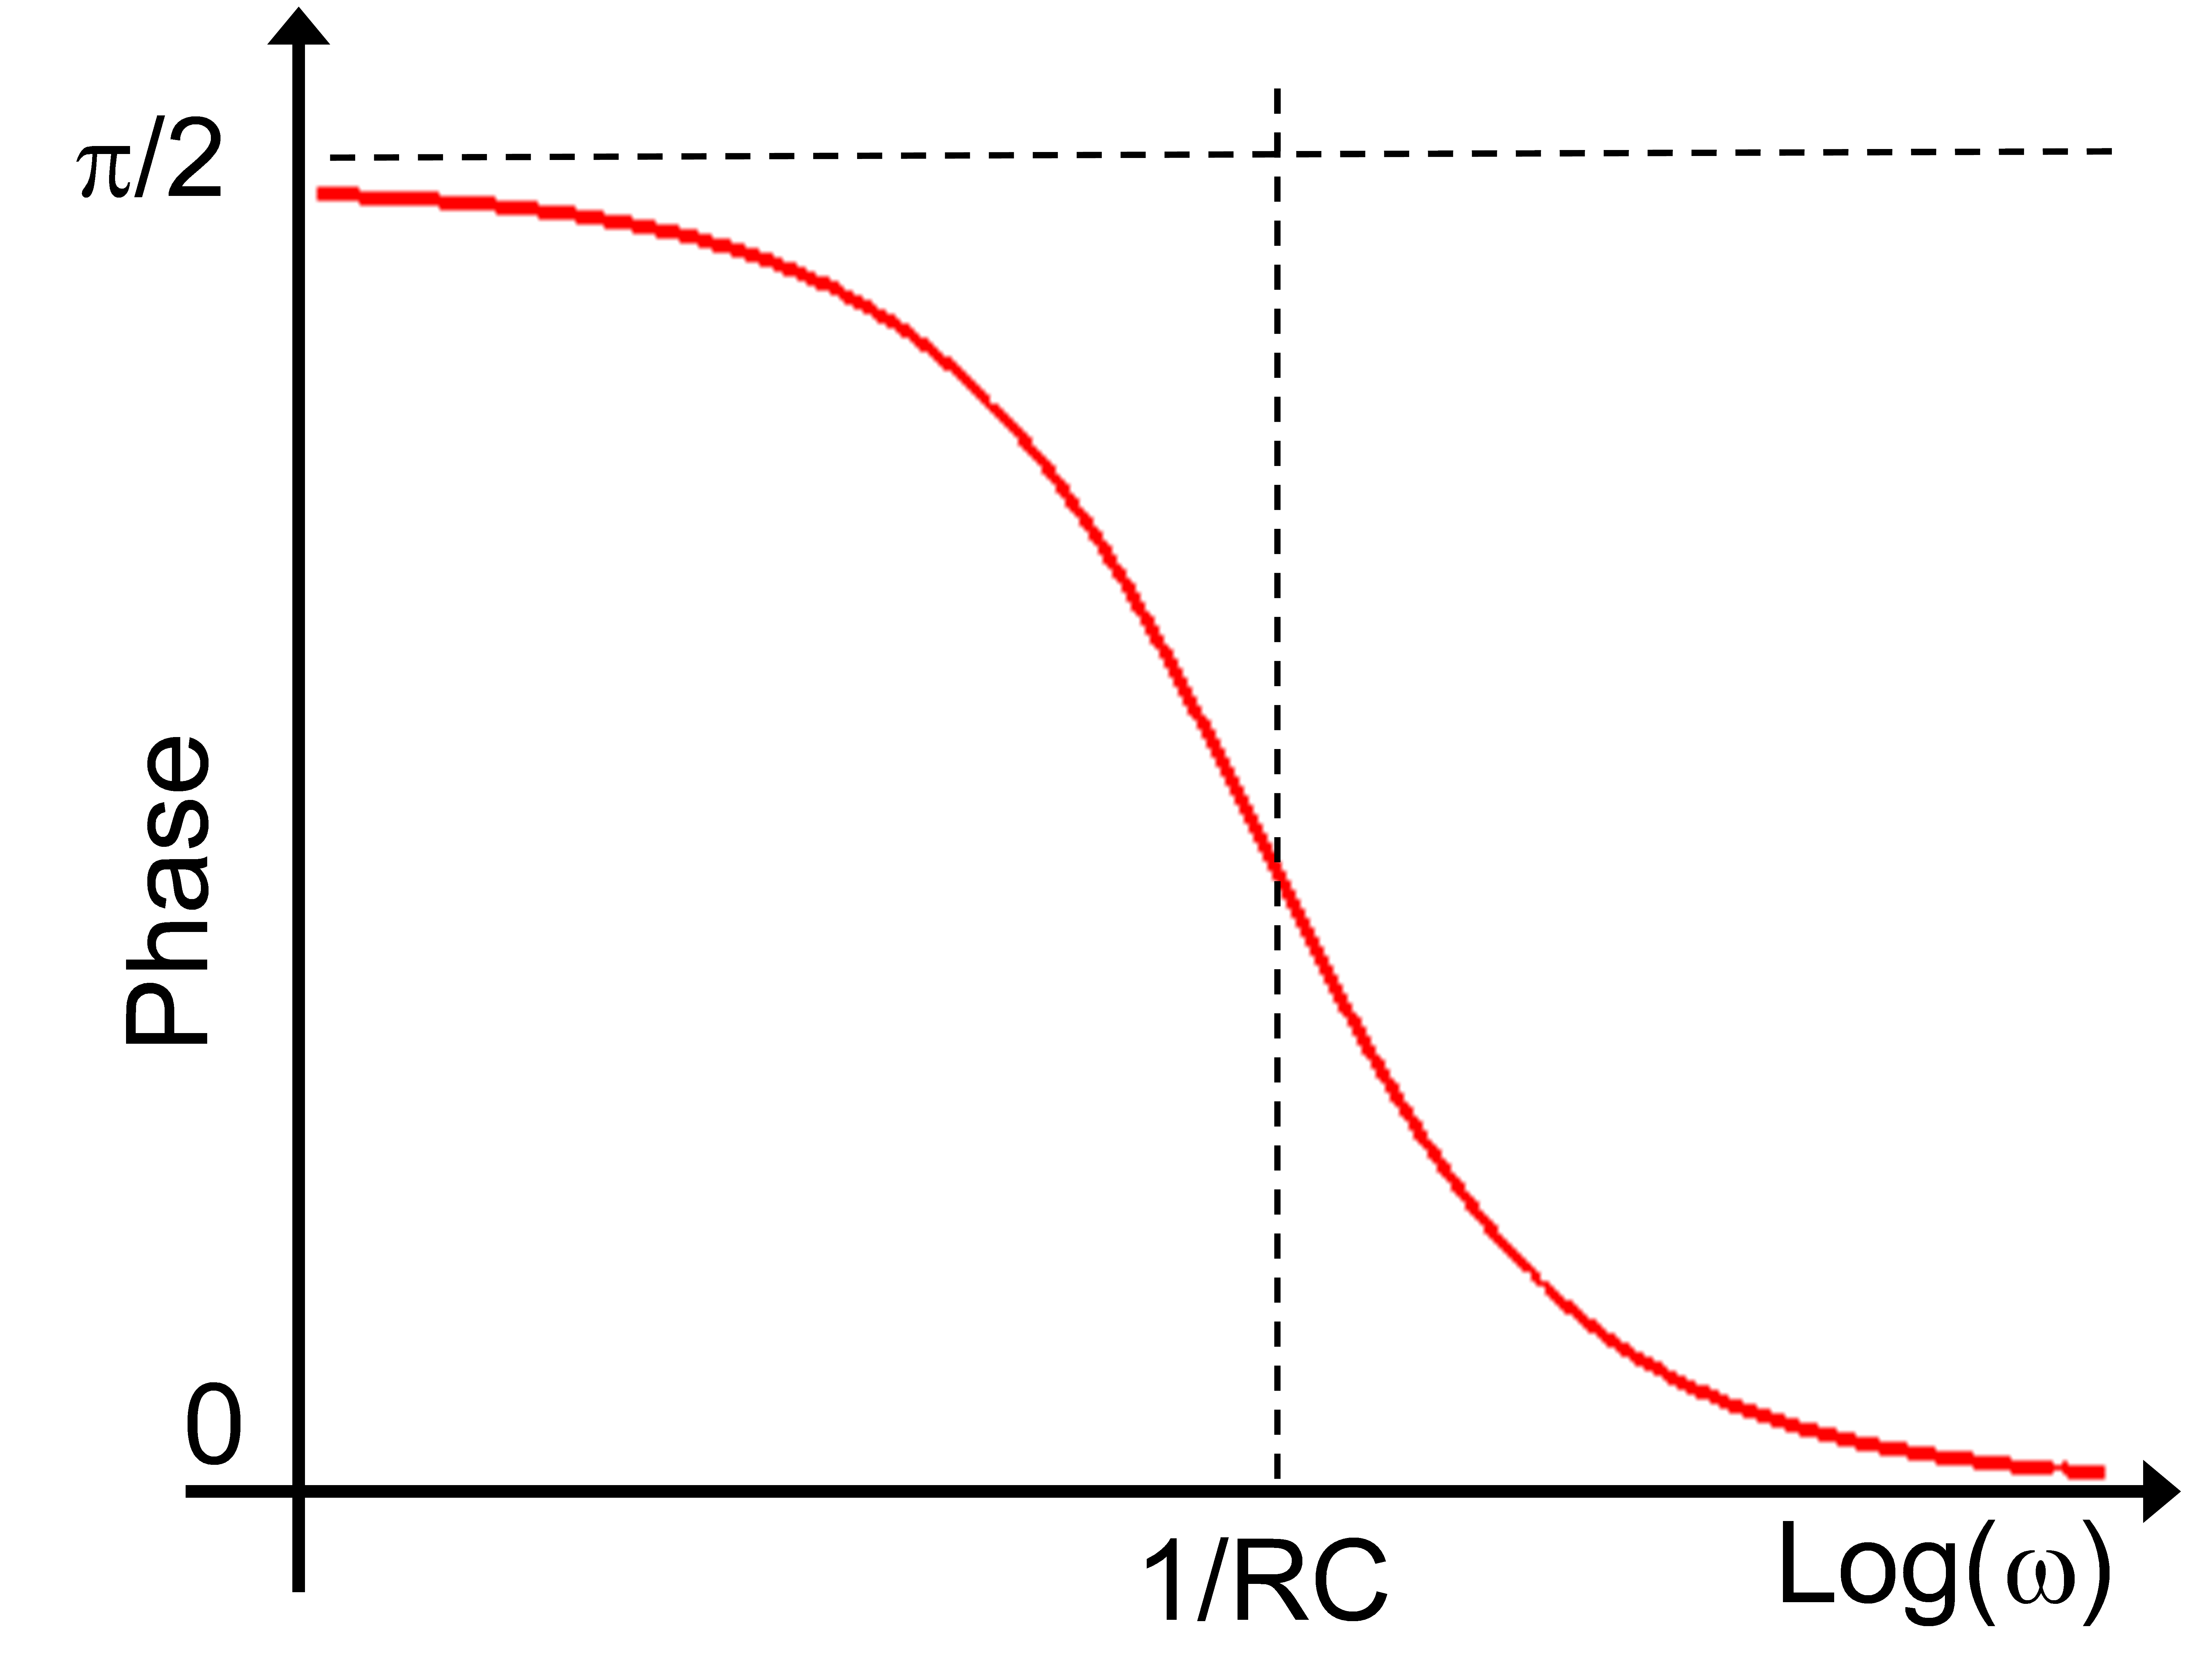
\includegraphics[width=0.45\textwidth]{pics/rc_high_pass_filter_bode_plot_phase}
\end{center}
\caption{Bode plots of the relative magnitude (left) and phase (right) of the output of an RC high-pass filter.}
\label{fig:rc_high_pass_filter_bode_plot}
\end{figure}

The Bode plots (log-log or semi-log plots) for the gain and phase of the high-pass filter are shown in figure 4.4, below. 

\subsubsection{RC Filter Design}

When designing an RC filter, you need to think about two things:
\begin{enumerate}
\item Choose an appropriate $f_{3\,dB}$.
\item Make sure the impedance is appropriate for your desired output load.
\end{enumerate}
Step 1 is straightforward and depends on the frequencies you want to pass and block.  In Step 2 you pick $R$ so as to satisfy the impedance requirements of your signal source and your signal destination. Typically, the signals we want to pass are around $f_{3\,dB}$, so the impedance of the capacitor and the impedance of the resistor will be about the same.

When filtering an input, choose the resistance to be about 10 times smaller than the input impedance of the next stage. This will prevent the next stage from loading the filter. You would also like to choose the resistance to be at least 10 times larger than the previous stage of your circuit's output impedance.
Choose the capacitor for the appropriate $f_{3\,dB} = 1/2\pi RC$
\begin{itemize}
\item If the signal you want to pass is low frequency, choose $f_{3\,db} \approx 2 f_{pass}$, and hence $C \approx 1/4\pi R f_{pass}$.
\item If the signal you want to pass is high frequency, choose $f_{3\,db} \approx f_{pass}/2$, and hence $C \approx 1/\pi R f_{pass}$.
\end{itemize}

\subsubsection{Combination Filters}
If you put several RC filters in a row you can make a more sophisticated signal filter. For example, several similar low-pass filters placed on after the other will produce a steeper fall off of the gain. One can also use a low-pass followed by a high pass to produce a bandpass filter ($f_{3\,dB,low-pass} > f_{3\,dB,high-pass}$).

\emph{Design tip}: When you are designing a bandpass filter, you should make sure that the resistor in the second stage is larger than the first stage by about a factor of 10. Otherwise, the second stage will load the first stage, and shift the effective $f_{3\,dB}$ frequency of the first stage.

\subsubsection{Applications}
Here are some specific applications of RC filters:

\paragraph{Blocking Capacitor}
This is a high pass filter that is used to eliminate DC. Suppose that you want to measure small time-dependent signals that happen to ``float'' on a high voltage. If you use a blocking capacitor, then the high voltage DC will not get through to your detection electronics, but the signal will get through. Choose $f_{3\,dB}$ low to ensure that your entire signal gets through.
 
\paragraph{Ripple Eliminator}
This is a low pass filter used to build power supplies. Since most of our power is 60\,Hz AC, our DC power supplies will convert AC to DC, but there will always be some residual 60\,Hz ``ripple''. A low pass filter with $f_{3\,dB}$ set well below 60\,Hz will work. You do not use a resistance in this case, but let the combination of the loading resistance $R_L$ and the Th\'{e}venin resistance of the previous components serve as your $R$. This usually requires a large capacitor since $R_L$ might be quite small when you use the power supply. If the capacitor is not big enough, then $f_{3\,dB}$ will then shift to a higher frequency, and the 60\,Hz ripple will reappear.

\paragraph{Chip Supply Clean-Up}
Frequently the voltage which you supply to a chip component, such as an op-amp (we will study these later in the semester), may be ``clean'' when it comes out of the power supply, but will pick up noise by the time it reaches the component. In this case a 10--100\,nF capacitor placed at the supply leads of the component will remove the high frequency pick-up noise.

\paragraph{Noise Eliminator}
Any signal line is susceptible to picking up high frequency transients; especially if there are motors or switching power supplies (or FM radio stations!) nearby. A noise eliminator is a low pass filter with a high value of $f_{3\,dB}$. 

\paragraph{Integrator}
If you build an $RC$ filter, but set the value of $f_{3\,dB}$ much higher than the highest frequency in your signal, the filter integrates your signal. From our earlier analysis, when $f \ll f_{3\,dB}$, we can see that each (low) frequency voltage component will see the same $\pi/2$ phase shift and its amplitude will be proportional to $1/f$. This is exactly the prescription for integration in Fourier space. So, a high pass filter sends high frequencies out on the resistor, and the integral of very low frequencies on the capacitor. 

\paragraph{Differentiator}
If you build an $RC$ filter with $f_{3\,dB}$ lower than the lowest frequency in your signal, the filter differentiates your signal. From our earlier analysis, when $f \gg f_{3\,dB}$, each (high) frequency voltage component will see the same $\pi/2$ phase shift and its amplitude will be proportional to $f$. This is exactly the prescription for differentiation in Fourier space. So, a low pass filter sends low frequencies out on the capacitor, and the derivative of high frequencies on the resistor.

\subsubsection{High frequency performance of capacitors}
In principle, one could use an $LR$ (inductor-resistor) circuit instead of an $RC$ circuit to make low-pass and high-pass filters and obtain similar performance. However, in practice one generally avoids inductors if possible. Inductors tend to be physically larger, more expensive, and deviate further from ideal performance than capacitors.

While capacitors generally offer superior performance to inductors, they also show significant deviations from the ideal impedance $Z_C = \frac{1}{j\omega C}$ at high frequencies. Capacitors will generally have a little bit of spurious resistance (i.e. like a resistor) and inductance (i.e. like an inductor) at high frequencies. In fact, circuit designers will often model a real capacitor with the following simple circuit, though more complex circuits are sometimes necessary, as shown in Figure~\ref{fig:real_capacitor}.

\begin{figure}
\begin{center}
\begin{circuitikz}
\draw (0,2) to[C,l=$C$,o-o] (2,2);
\draw (-2,0) to[C,l=$C$,o-] (0,0) to[R,l=$R$ (small)] (2,0) to[L,l=$L$ (small),-o] (4,0);
\end{circuitikz}
\end{center}
\caption{A real capacitor can be modeled as an ideal capacitor in series with some small resistor and inductor.}
\label{fig:real_capacitor}
\end{figure}

\begin{figure}
\begin{center}
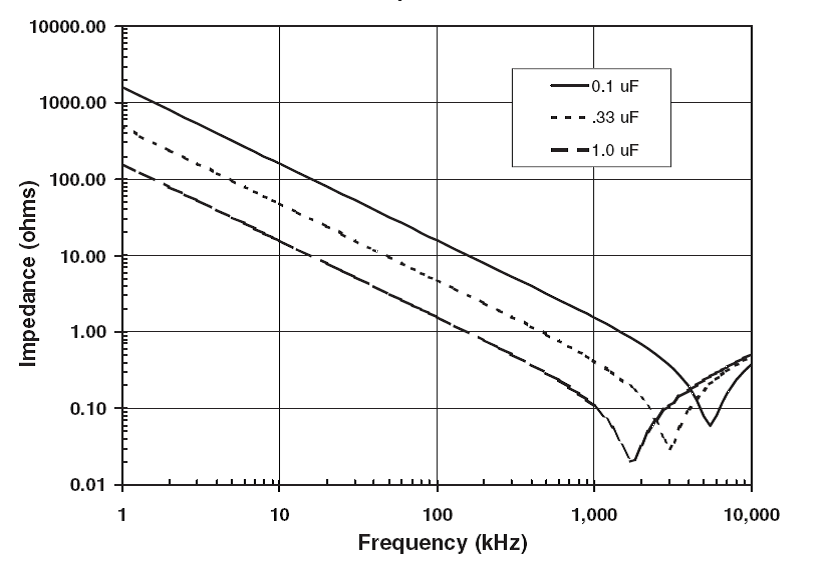
\includegraphics[width=0.45\textwidth]{pics/capacitor_cornell_dubilier}
\end{center}
\caption{Impedance of real capacitors versus frequency. Note that the capacitors behave like inductors above a few MHz [source: Cornell Dubilier].}
\label{fig:capacitor_cornell_dubilier}
\end{figure}

The resistance is due to the non-zero high frequency conductivity of the dielectric material separating the two conductor plates of the capacitor. The inductance is due to two effects: 1) the design of the capacitor, especially the leads, will contribute inductance., and 2) Maxwell's equations for electrodynamics require that a capacitor have an inductance at high frequencies\footnote{The Feynman Lectures on Physics, Vol. 2, by R. P. Feynman, R. B. Leighton, and M. Sands, p. 23-2}. Capacitor manufacturer will provide the specifications for the spurious resistance and inductance of their capacitors. The plot in Figure~\ref{fig:capacitor_cornell_dubilier}, below, shows the frequency dependence of the impedance of a Cornell Dubilier acrylic surface mount film capacitor.

A common remedy for dealing with the inherent inductance of a capacitor at high frequencies is to place a small capacitor (10--100 pF) in parallel with the main capacitor in RC filter. The high frequency performance of the small capacitor will generally much better than that of the main capacitor: the small will pick-up the high frequency signal when the main, larger capacitor begins to have a significant inductance. The gain fall-off of the $RC$ filter will no longer be -20 dB/decade, but at least a low-pass filter will not start to behave like a high-pass filter (or vice-versa)!


\subsection{$LC$ Filters}
Although $RC$ filters are by far the simplest and the most common type of filter found in analog circuits, they suffer from a relatively slow roll off of the gain: while the gain or attenuation slope can be made steeper than -20\,dB/decade, the transition region, or knee of the curve (the region where the gain changes from flat to a log-log slope), will always have the same shape and frequency width.

$LC$ filters are more complex but can be engineered to produce much sharper features and steeper fall-off regions. The standard design for $LC$ filters is an $LC$ ladder with an un-interrupted ground line, such as in the 5th order filters shown in Figure~\ref{fig:lc_low_pass_filter_5th_order} and \ref{fig:lc_low_pass_filter_5th_order} below:

\begin{figure}
\begin{center}
\begin{circuitikz}
\draw (1,2) to[short,o-] (2,2) to[C,l=$C_1$] (2,0) to[short,-o] (1,0);
\draw (2,2) to[L,l=$L_1$] (4,2) to[C,l=$C_2$] (4,0) to[short] (2,0);
\draw (4,2) to[L,l=$L_2$] (6,2) to[C,l=$C_3$] (6,0) to[short] (4,0);
\draw (6,2) to[L,l=$L_3$] (8,2) to[C,l=$C_4$] (8,0) to[short] (6,0);
\draw (8,2) to[L,l=$L_4$] (10,2) to[C,l=$C_5$] (10,0) to[short] (8,0);
\draw (10,2) to[short,-o] (11,2);
\draw (10,0) to[short,-o] (11,0);
\end{circuitikz}
\end{center}
\caption{5th order low-pass LC filter.}
\label{fig:lc_low_pass_filter_5th_order}
\end{figure}

\begin{figure}
\begin{center}
\begin{circuitikz}
\draw (1,2) to[short,o-] (2,2) to[L,l=$L_1$] (2,0) to[short,-o] (1,0);
\draw (2,2) to[C,l=$C_1$] (4,2) to[L,l=$L_2$] (4,0) to[short] (2,0);
\draw (4,2) to[C,l=$C_2$] (6,2) to[L,l=$L_3$] (6,0) to[short] (4,0);
\draw (6,2) to[C,l=$C_3$] (8,2) to[L,l=$L_4$] (8,0) to[short] (6,0);
\draw (8,2) to[C,l=$C_4$] (10,2) to[L,l=$L_5$] (10,0) to[short] (8,0);
\draw (10,2) to[short,-o] (11,2);
\draw (10,0) to[short,-o] (11,0);
\end{circuitikz}
\end{center}
\caption{5th order high-pass LC filter.}
\label{fig:lc_high_pass_filter_5th_order}
\end{figure}

The algebra required for computing the gain and phase Bode plots for these filters is generally quite cumbersome, and a computer program (i.e. Maple or Excel) is generally useful for helping with the design. A number of web-applets can also be found on the internet for determining all the inductor and capacitor values that will produce the required filter performance.

Example 1: 5th order Butterworth $LC$ low-pass filter with $f_{3\,dB} = 10$\,kHz for 50\,\Ohm input impedance and 50\,\Ohm output impedance. The relative amplitude of the output is shown in Figure~\ref{fig:lc_low_pass_butterworth_filter_5th_order}.

\begin{figure}
\begin{center}
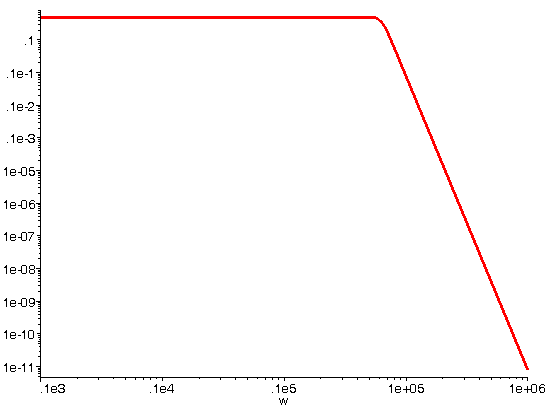
\includegraphics[width=0.45\textwidth]{pics/lc_low_pass_butterworth_filter_5th_order}
\end{center}
\caption{Bode plot of the gain of a 5th order Butterworth $LC$ low-pass filter.}
\label{fig:lc_low_pass_butterworth_filter_5th_order}
\end{figure}

This Butterworth filter uses $C_1 = C_5 = 0.6946\,\mu$F, $C_2 = C_4 = 3.0642\,\mu$F, $C_3 = 4\,\mu$F, $L_1 = L_4 = 5$\,mH, and $L_2 = L_3 = 9.397$\,mH. Butterworth filters have a very flat pass-band, and a reasonably regular phase change across the knee of the curve.

Example 2: 5th order Chebyshev LC low-pass filter with $f_{3\,dB} = 10$\,kHz for 50\,\Ohm input impedance and 50\,\Ohm output impedance. The relative amplitude of the output is shown in Figure~\ref{fig:lc_low_pass_chebyshev_filter_5th_order}.


\begin{figure}
\begin{center}
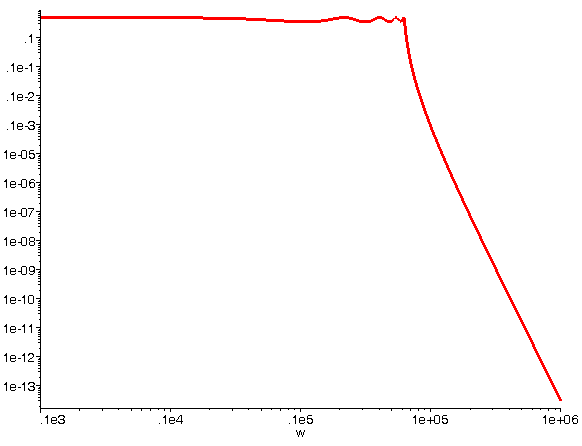
\includegraphics[width=0.45\textwidth]{pics/lc_low_pass_chebyshev_filter_5th_order}
\end{center}
\caption{Bode plot of the gain of a 5th order Chebyshev $LC$ low-pass filter.}
\label{fig:lc_low_pass_chebyshev_filter_5th_order}
\end{figure}

This Chebyshev filter uses $C_1 = C_5 = 1.125\,\mu$F, $C_2 = C_4 = 1.486\,\mu$F, $C_3 = 1.505\,\mu$F, $L_1 = L_4 = 0.617$\,mH, and $L_2 = L_3 = 0.646$\,mH. Chebyshev filters have a very sharp knee and fast cut-off, but suffer from irregular transmission in the pass-band. They also have a highly irregular phase variation at the knee of the filter.

The above Chebyshev and Butterworth filters can be scaled to another frequency or load impedance with the following rules:
\begin{eqnarray}
L_{new} & = & \frac{R_{load,new}}{R_{load,old}} \frac{f_{3\,dB,old}}{f_{3\,dB,new}} L_{old}, \\
C_{new} & = & \frac{R_{load,old}}{R_{load,new}} \frac{f_{3\,dB,new}}{f_{3\,dB,old}} C_{old}.
\end{eqnarray}


\subsubsection{Some remarks on $LC$ filters}
\begin{enumerate}
\item Generally, the higher the order of the $LC$ filter, the sharper the cut-off will be, however this usually requires a trade-off in the regularity of the output phase.
\item $LC$ filters do not have resistive elements, and consequently they do not consume power, and do not load the source signal. However, the load of the input device into which the filter sends its output will load the $LC$ filter and can shift the $f_{3\,dB}$ point considerably---always remember to include the load resistor in your calculations.
\item $LC$ filters are widely used in RF circuits, where active filters do not have the bandwidth to respond to high frequencies.
\item One cannot construct a filter with arbitrary gain and phase profiles. While we have treated filters in Fourier space, in the time domain filters must obey causality. In fact, one can derive Kramers-Kronig relations for filters.
\end{enumerate}

\section{Transmission Lines}
Signals are sent from one device to another, or from one part of a circuit to another with transmission lines. The quality of your transmission determines the quality of your signal, whether you are connecting one device to another or a resistor to a capacitor.

\subsection{LC Ladder Model of a Transmission Line}
A transmission line consists of two parallel conductors separated by a fixed distance $d$, which gives rise to an effective capacitance $C$ per unit length. The conductors will also produce a magnetic field, which is gives the transmission line an effective inductance $L$ per unit length. We can model the transmission line as a repeated network of series inductors and parallel capacitors, or $LC$ ladder, as depicted in the Figure~\ref{fig:transmission_line}.

\begin{figure}
\begin{center}
\begin{circuitikz}
\draw (1,2) to[short,o-] (2,2) to[C,l=$C$] (2,0) to[short,-o] (1,0);
\draw (2,2) to[L,l=$L$] (4,2) to[C,l=$C$] (4,0) to[short] (2,0);
\draw (4,2) to[L,l=$L$] (6,2) to[C,l=$C$] (6,0) to[short] (4,0);
\draw (6,2) to[L,l=$L$] (8,2) to[C,l=$C$] (8,0) to[short] (6,0);
\draw (8,2) to[short] (9,2);
\draw (8,0) to[short] (9,0);
% gap needs ldots
\draw (10,2) to[L,l=$L$] (12,2) to[C,l=$C$] (12,0) to[short] (10,0);
\draw (12,2) to[L,l=$L$,-o] (14,2);
\draw (12,0) to[short,-o] (14,0);
\end{circuitikz}
\end{center}
\caption{A transmission line modeled with capacitors and inductors.}
\label{fig:transmission_line}
\end{figure}

If the $LC$ ladder is infinite and has an impedance $Z_0$, then if we add an extra $LC$ ladder ``rung'', the total impedance should not change, and we obtain the following relation
\begin{equation}
Z_0 = (L + Z_0) \parallel C
\end{equation}
or
\begin{equation}
Z_0 = \frac{(j\omega L + Z_0) \frac{1}{j\omega C}}{j\omega L + Z_0 + \frac{1}{j\omega C}}
\end{equation}
From this relation we can extract an expression for $Z_0$, and we obtain
\begin{equation}
Z_0 = \frac{1}{2} j\omega L + \sqrt{\frac{L}{C} - \frac{1}{4}\omega^2 L^2}
\end{equation}
If we consider that $L$ and $C$ are the inductance and capacitance, respectively, of a short section $\Delta\ell$ of transmission line, then as we take the limit $\Delta\ell \to 0$ we have $L \to 0$ and $C \to 0$, but $L/C$ constant. In this limit the equation for $Z_0$ becomes
\begin{equation}
Z_0 = \sqrt{\frac{L}{C}}
\end{equation}
where $L$ and $C$ are the inductance and capacitance, respectively, of the transmission line, and $Z_0$ is called the characteristic impedance of the transmission line.

It may seem surprising that a network of inductors and capacitors can have a real impedance, and consequently consume power. The explanation for this apparent paradox is that since the network is infinite, power is flowing from one $LC$ ladder rung to the next ad infinitum, so that power is constantly moving down the transmission line, though it is not dissipated in either the inductors or capacitors. Of course, the power is consumed at the end of the transmission line when we attach a load resistor.

The $LC$ ladder model is a high frequency model of transmission line and does not include the wire resistance which can contribute to signal attenuation. 

\subsection{Transmission Line Impedance Matching}
A transmission line with a characteristic impedance of $Z_0$ should be terminated with a load impedance of $Z_0$ if the transmission line is longer than 1/10 of the wavelength of the signal (recall $\lambda = c/f$, where $c$ is the speed of light in the transmission line and $f$ is the signal frequency). If the transmission line is not properly terminated, then the signal will be partially reflected back towards the source upon arrival at the load.

There are three main types of transmission lines: wires, twisted pairs, and coaxial cables. In this section we go over their performance characteristics.

\paragraph{Wires}
Plain wires are the simplest and the cheapest transmission lines available: they include the wires you use to connect components on your breadboard and electrical grid power lines. If the wires are kept parallel, then the transmission line will provide some protection to external fields and noise at low frequencies. While wire transmission lines are simple, they should be avoided whenever possible since they are susceptible to interference and high frequency pick-up. At high frequencies a wire transmission line actually becomes an antenna (for both transmission and reception).

\paragraph{Twisted Pairs}
A twisted pair of wires provides good protection from outside fields and noise and can transmit relatively high frequency signals without difficulty. The electromagnetic field of a signal kept close to the wire pair. A twisted pair can transmit analog signals at up to 250\,kHz (sometimes even 1\,MHz) and digital signals up to 100\,MHz. Twisted pairs are quite common and are used in many computer communications cable, such as RJ45 Ethernet cables which has a characteristic impedance of $Z_0 = 100$\,\Ohm. Twisted pair transmission lines are easy to make: just take two wires of equal length and twist them together!

\paragraph{Coaxial Cables}
Coaxial cable is the best form of transmission line, short of a waveguide. In the limit of perfect conductors, signals on coaxial cables are impervious to external fields and do not radiate either. Coaxial cables can be used for frequencies up to 1\,GHz. At high frequencies, a significant fraction of the transmitted energy/power is in the electric and magnetic fields that carry the signal though the cable, instead of in the potential energy of the current carrying electrons. The speed of light in a coaxial cable is usually 60-70\% of the speed of light in vacuum. The characteristic impedance of most coaxial cables used in industry and labs is $Z_0 = 50$\,\Ohm---coaxial cable for cable TV is an exception, it has a characteristic impedance of 75\,\Ohm.


\pagebreak

\section{Lab 4: Design Exercises}
\begin{enumerate}
\item Design a high-pass $RC$ filter that can filter out 60\,Hz and 120\,Hz but yet still pass signals above 10\,kHz. This filter should work with a load of at least 100\,k\Ohm. You can assume that your signal source has a 50\,\Ohm impedance or lower. Plot the amplitude transfer function of this filter in dB, mark the 3\,dB point.

\item Design a band-pass filter which will only pass frequencies near 10\,kHz ($G(10\,\hbox{kHz}) > 0.90$) and filter frequencies below 1\,kHz and above 100\,kHz. This filter should work with a load of at least 100\,k\Ohm. You can do this by combining two different $RC$ filters (one high pass and one low pass). You can assume that your signal source has a 50\,\Ohm impedance or lower. Plot the amplitude transfer function of this filter in dB, mark the 3\,dB points.
\end{enumerate}

\section{Lab 4: Passive Filters}

\subsection{Source Impedance Review (30 minutes)}
\begin{enumerate}
\item Set the output of the function generator to a 1\,Hz (or less) square wave with a voltage which varies between 0\,V and 5\,V. Make sure that lower part of the square wave is as close to 0\,V as possible. Try to use the output of the function generator to power a light bulb (if you do not see any light, then increase the voltage until you do).
\item Measure the output voltage versus time when loaded by the light bulb. Is the output voltage consistent with what you would expect for a source with a 50\,\Ohm impedance driving a light bulb? Explain.
\end{enumerate}

\subsection{High-Pass Filter (1 hour)}
\begin{enumerate}[resume]
\item Design and construct a high-pass $RC$ filter that can filter out  60\,Hz but still pass signals in the kHz region. The one from design exercises is a good one to start.
\item Connect a 100\,kHz output from your signal generator to one terminal of the 6.3\,V transformer on your breadboard. This will add a large 60\,Hz noise component onto the signal. Your filter should be able to clean it up.  If your breadboard does not have a transformer, consider how else you can pick up 60\,Hz noise.
\item Measure the ratio of signal to noise (S/N) at the input and output, and compare it to your calculations, where ``signal'' is the peak-to-peak amplitude of the 100\,kHz sine wave, and ``noise'' is the peak-to-peak amplitude of the  60\,Hz component.
\end{enumerate}

\subsection{Band-Pass Filter (1 hour)}
\begin{enumerate}[resume]
\item Design and construct a band-pass filter which will only pass frequencies near 10\,kHz. (You can do this by combining 2 different $RC$ filters. See design exercises.)
\item Measure its response/transfer function (amplitude ratio and phase difference) when driving a load of 100\,k\Ohm at 50\,Hz, 100\,Hz, 1\,kHz, 5\,kHz, 10\,kHz, 20\,kHz, 50\,kHz, 100\,kHz and 1\,MHz. Does your circuit behave the way you expect it to? 
\item Now connect 1\,k\Ohm load to your filter. Measure its response at the same frequencies. Is it the same as before? Explain.
\end{enumerate}

\end{document}
